%%% -*- TeX-master: "../main" -*-
\chapter{Results}
\label{cha:results}

We trained neural networks on each of the three sequence representations, the
preprocessed event stream, gists and CNN features from the InceptionV3 network,
with each of CTC and cross entropy losses. The training progress for all
combinations is depicted in Figure \ref{fig:losses}. The first thing that
strikes the eye is that the classification of InceptionV3 features did not work
at all. The training error decreases but the validation error either moves
randomly or only ever decreases. This is indicative that the extracted features
are not meaningful and the network can only memorize the input instead of
understanding patterns. The problem can most likely be traced back to the
quality of the frame reconstructions which also have to be scaled by a factor of
\textasciitilde 2.3.

The other representations both show the normal training progression one would
expect. In the beginning both training and validation error decrease almost
equally, and at some point the validation error stalls or begins to slightly
increase as the network overfits the training set. The latter effect is very
pronounced in Figures \ref{fig:losses-ce-gists}, \ref{fig:losses-ce-events} and
\ref{fig:losses-ctc-events}. The plots show that the gist representation allows
a network to reach a lower average loss per epoch on the validation set with
either loss function, cross entropy or CTC. The networks were trained for
different numbers of epochs because of the different costs of training a
network. Gists and CNN features compress a sequence of events by a factor of
about a hundred in the time dimension, so subsequent classifier networks can be
trained in about five minutes per epoch on a Titan X graphics card. Training on
the event data takes about half an hour per epoch.

All networks exhibit a relatively large generalization gap at the point of
minimum validation loss. This leads us to believe that regularization is viable
here, though exploring that is outside the scope of this thesis.

Next, we selected the network with minimum validation loss in each of the six
categories to classify the event sequences in the validation set. This opens us
up to a kind of overfitting on the validation set because we measure the
generalizability with the classifier of which we know beforehand that it
performs best. In the best case we would have had a test set recorded from a
person whose recordings are not part of the training data at all. However, we
think that assessing the performance on the validation set is still indicative
of the true generalizability because, after all, no component of the recognition
pipeline has seen the validation data directly during training.

After applying the classifiers, we derived the HMM parameters from the training
data as described in the previous chapter. Before presenting the results, we
will have to explain how we assess recognition performance. The measure used by
Graves for sequence labelling is the label error rate (LER). It is based on the
Levenshtein distance between two sequences. Let $(a_{i})$ and $(b_{j})$ be two
label sequences. Then the Levenshtein or edit
\begin{figure}[H]
  \begin{subfigure}[t]{3in}
  \centering
    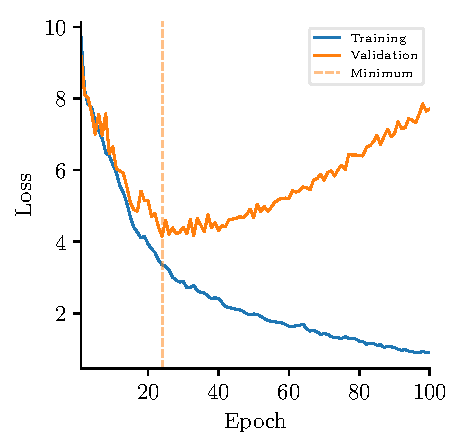
\includegraphics[width=2.5in]{figures/results/losses/gru-gists}
    \caption{Cross entropy training on gists}
    \label{fig:losses-ce-gists}
  \end{subfigure}
  \hfill
  \begin{subfigure}[t]{3in}
  \centering
    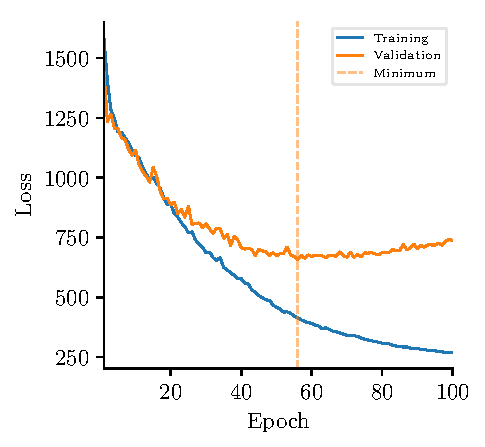
\includegraphics[width=2.5in]{figures/results/losses/ctc-gists}
    \caption{CTC training on gists}
    \label{fig:losses-ctc-gists}
  \end{subfigure}
  \begin{subfigure}[t]{3in}
  \centering
    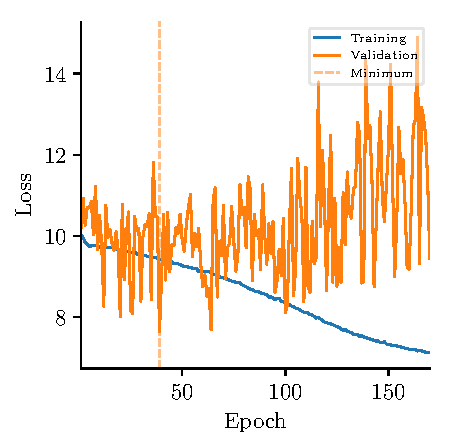
\includegraphics[width=2.5in]{figures/results/losses/gru-inceptionv3}
    \caption{Cross entropy training on InceptionV3 features}
    \label{fig:losses-ce-iv3}
  \end{subfigure}
  \hfill
  \begin{subfigure}[t]{3in}
  \centering
    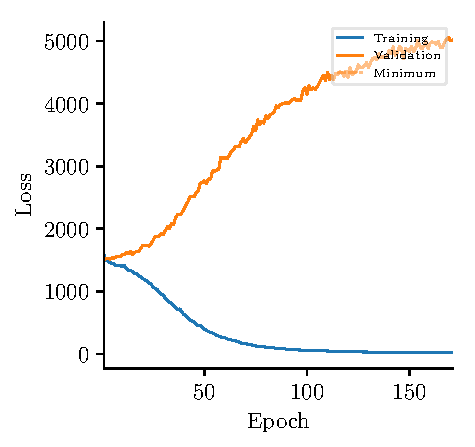
\includegraphics[width=2.5in]{figures/results/losses/ctc-inceptionv3}
    \caption{CTC training on InceptionV3 features}
    \label{fig:losses-ctc-iv3}
  \end{subfigure}
  \begin{subfigure}[t]{3in}
  \centering
    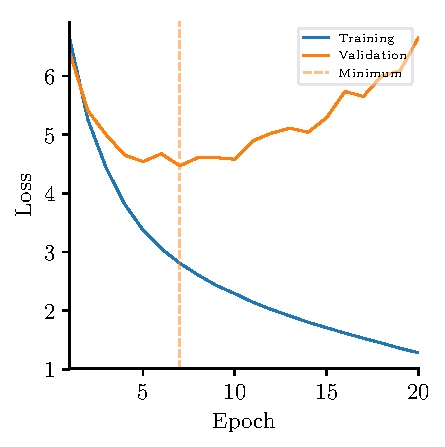
\includegraphics[width=2.5in]{figures/results/losses/gru-events}
    \caption{Cross entropy training on events}
    \label{fig:losses-ce-events}
  \end{subfigure}
  \hfill
  \begin{subfigure}[t]{3in}
  \centering
    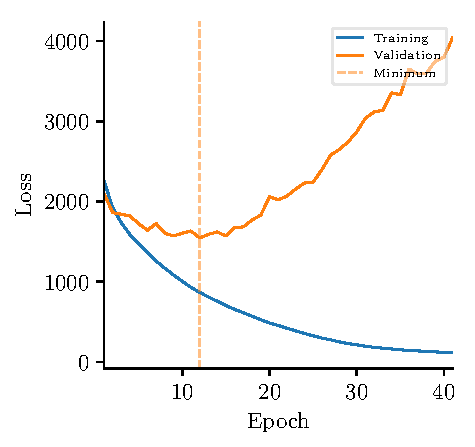
\includegraphics[width=2.5in]{figures/results/losses/ctc-events}
    \caption{CTC training on events}
    \label{fig:losses-ctc-events}
  \end{subfigure}
  \caption{Progression of losses on the training and validation set. The dashed
    line marks the epoch of minimum validation loss.}
  \label{fig:losses}
\end{figure}
\noindent
distance $\mathrm{ED}(a, b)$ between the two sequences is the minimum number of
insert, remove and replace operations needed to change one sequence into the
other. This is illustrated in Figure \ref{fig:levenshtein} which shows the label
sequence of a recording and what our system recognized side by side. The
Levenshtein distance between them is 3 because two labels need to be replaced
and one removed. The label error rate is defined in terms of the edit distance
as
\begin{equation*}
  \mathrm{LER} = \frac{1}{\sum_{(l, l') \in Z} |l|} \sum_{(l, l') \in Z} \mathrm{ED}(l, l')
\end{equation*}
where $Z$ is the set of all true label sequences $l$ and predicted label
sequences $l'$ in a dataset, in our case the validation dataset. So the LER is
the average number of edit operations necessary per true label. If the number of
insert and remove operations is small, $1 - \mathrm{LER}$ can informally be
treated as an accuracy of the recognition system because in that case the LER is
dominated by misclassifications.

\begin{figure}[h]
  \centering
  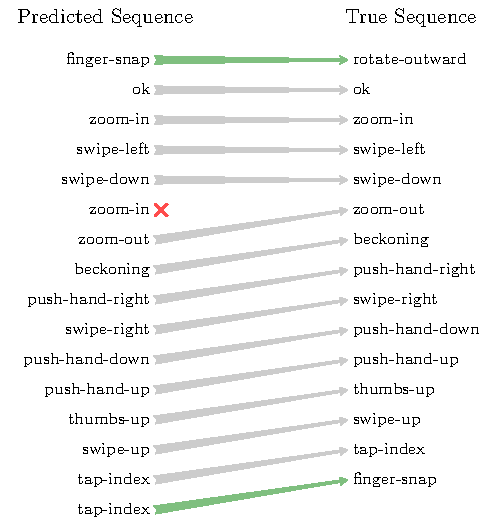
\includegraphics{figures/results/levenshtein}
  \caption{Decoded gesture sequence with a Levenshtein distance of 3 to the
    ground truth}
  \label{fig:levenshtein}
\end{figure}

Table \ref{tab:ler} presents the final results across all twelve combinations of
loss function, input representation and decoding method in the form of mean
Levenshtein distance and label error rate. The best result was achieved on gists
with a network trained for framewise classfication and decoding method with an
extra segmentation step. The mean Levenshtein distance is just 2, so of the 16
gestures shown in each of the recording it gets 14 correct on average, which is
an LER of 0.125 and an accuracy of 87.5\%. The accuracy interpretation is
approximately correct in this case because the network gets the number of
gestures wrong only a single time.

\begin{table}[h]
  \centering
  \begin{subtable}{\textwidth}
    \centering
    \begin{tabular}{r|c|c|c}
      % BEGIN RECEIVE ORGTBL levenshtein
Method & Events & Gists & InceptionV3\\
\hline
CE + HMM Segmentation & 6.5 & \textbf{2.0} & 14.5\\
CTC + HMM Segmentation & 16.0 & 12.5 & 15.25\\
CE + HMM Decoding & 2104.0 & 22.0 & 16.0\\
CTC + HMM Decoding & 3378.25 & 21.0 & 16.0\\
      % END RECEIVE ORGTBL levenshtein
    \end{tabular}
    \caption{Mean Levenshtein Distance (lower is better)}
  \end{subtable}
  \par\bigskip
  \begin{subtable}{\textwidth}
    \centering
    \begin{tabular}{r|c|c|c}
      % BEGIN RECEIVE ORGTBL label-error-rate
Method & Events & Gists & InceptionV3\\
\hline
CE + HMM Segmentation & 0.406 & \textbf{0.125} & 0.906\\
CTC + HMM Segmentation & 1.0 & 0.781 & 0.953\\
CE + HMM Decoding & 131.5 & 1.375 & 1.0\\
CTC + HMM Decoding & 211.14 & 1.313 & 1.0\\
      % END RECEIVE ORGTBL label-error-rate
    \end{tabular}
    \caption{Label Error Rate (lower is better)}
  \end{subtable}
  \caption{Performance measured on the validation set}
  \label{tab:ler}
\end{table}
\begin{comment}
  #+ORGTBL: SEND levenshtein orgtbl-to-latex :splice t
  | Method                 |  Events |        Gists | InceptionV3 |
  |------------------------+---------+--------------+-------------|
  | CE + HMM Segmentation  |     6.5 | \textbf{2.0} |        14.5 |
  | CTC + HMM Segmentation |    16.0 |         12.5 |       15.25 |
  | CE + HMM Decoding      |  2104.0 |         22.0 |        16.0 |
  | CTC + HMM Decoding     | 3378.25 |         21.0 |        16.0 |
\end{comment}
\begin{comment}
  #+ORGTBL: SEND label-error-rate orgtbl-to-latex :splice t
  | Method                 | Events |          Gists | InceptionV3 |
  |------------------------+--------+----------------+-------------|
  | CE + HMM Segmentation  |  0.406 | \textbf{0.125} |       0.906 |
  | CTC + HMM Segmentation |    1.0 |          0.781 |       0.953 |
  | CE + HMM Decoding      |  131.5 |          1.375 |         1.0 |
  | CTC + HMM Decoding     | 211.14 |          1.313 |         1.0 |
\end{comment}

All other combinations perform significantly worse, though segmentation improves
the label error rate in every case over simple decoding. To understand why that
is compare the plots in figure \ref{fig:decoded}. The direct decoding method has
16 non-blank states that each compete to explain the current frame
classification. This produces many spurious labels that are only active for a
few tenth of a second which in turn drives the Levenshtein distance up with a
lot of removal operations. The segmentation-HMM combines all gestures into one
non-blank class and is thus able to combine clusters of activations into one
segment which is subsequently assigned a single label. The problem is only
exacerbated when the pipeline is applied to the event representation. The cause
for the dramatically degraded performance on events when comparing a decoder to
the segmentation method is that HMMs model discrete time-series but event
sequences are continuous. Also our parameter estimation procedure for HMMs does
not account for the varying event densities between gesture and blank. As a
result, the HMM ``sees'' the gestures very drawn out which makes it easy to take
the noise in the event classification (see Figure \ref{fig:event-cls}) for a
true signal, if we anthropomorphize the inner workings of an HMM.

\begin{figure}[h]
  \centering
  \begin{subfigure}{\textwidth}
    \centering
    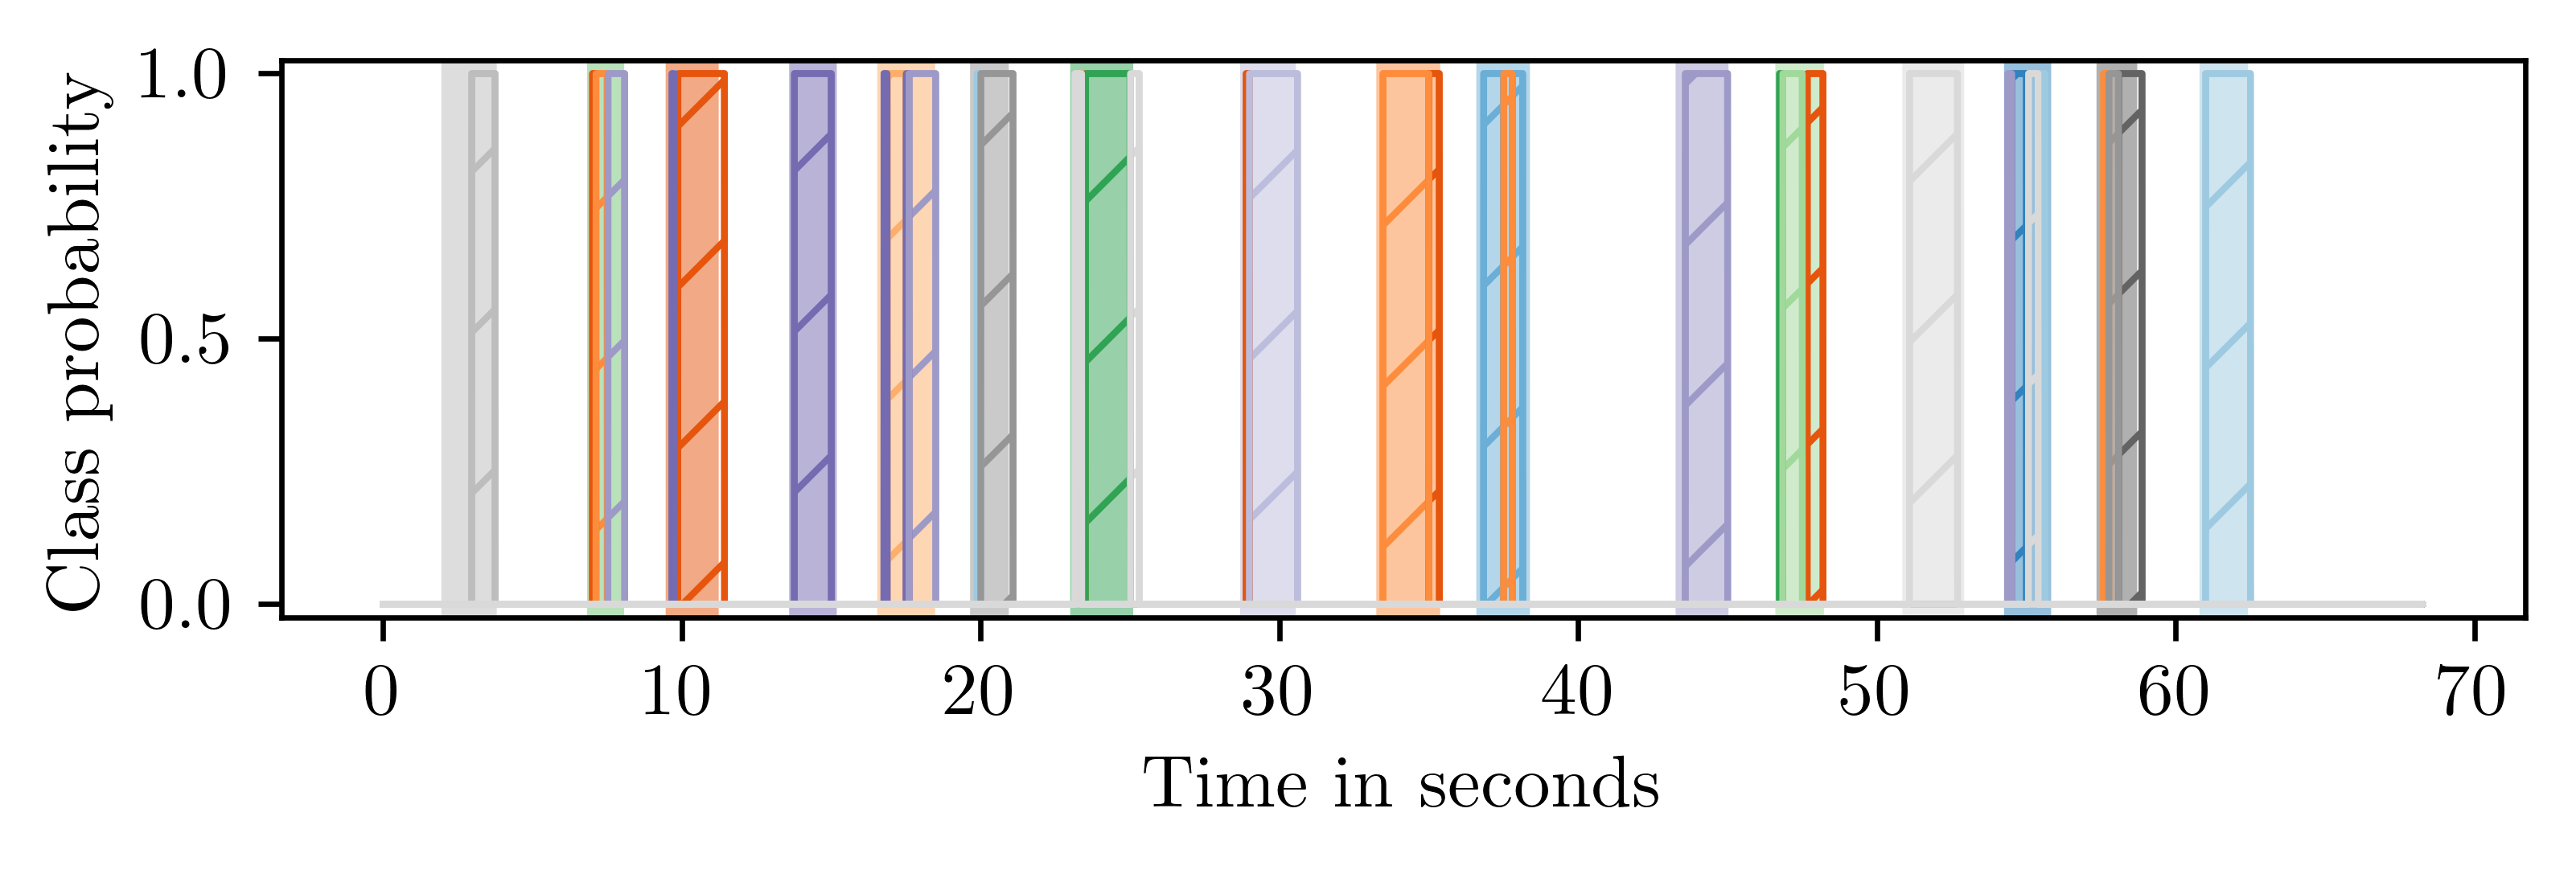
\includegraphics{figures/results/decoded/decoded}
    \caption{Direct HMM decoding}
  \end{subfigure}
  \begin{subfigure}{\textwidth}
    \centering
    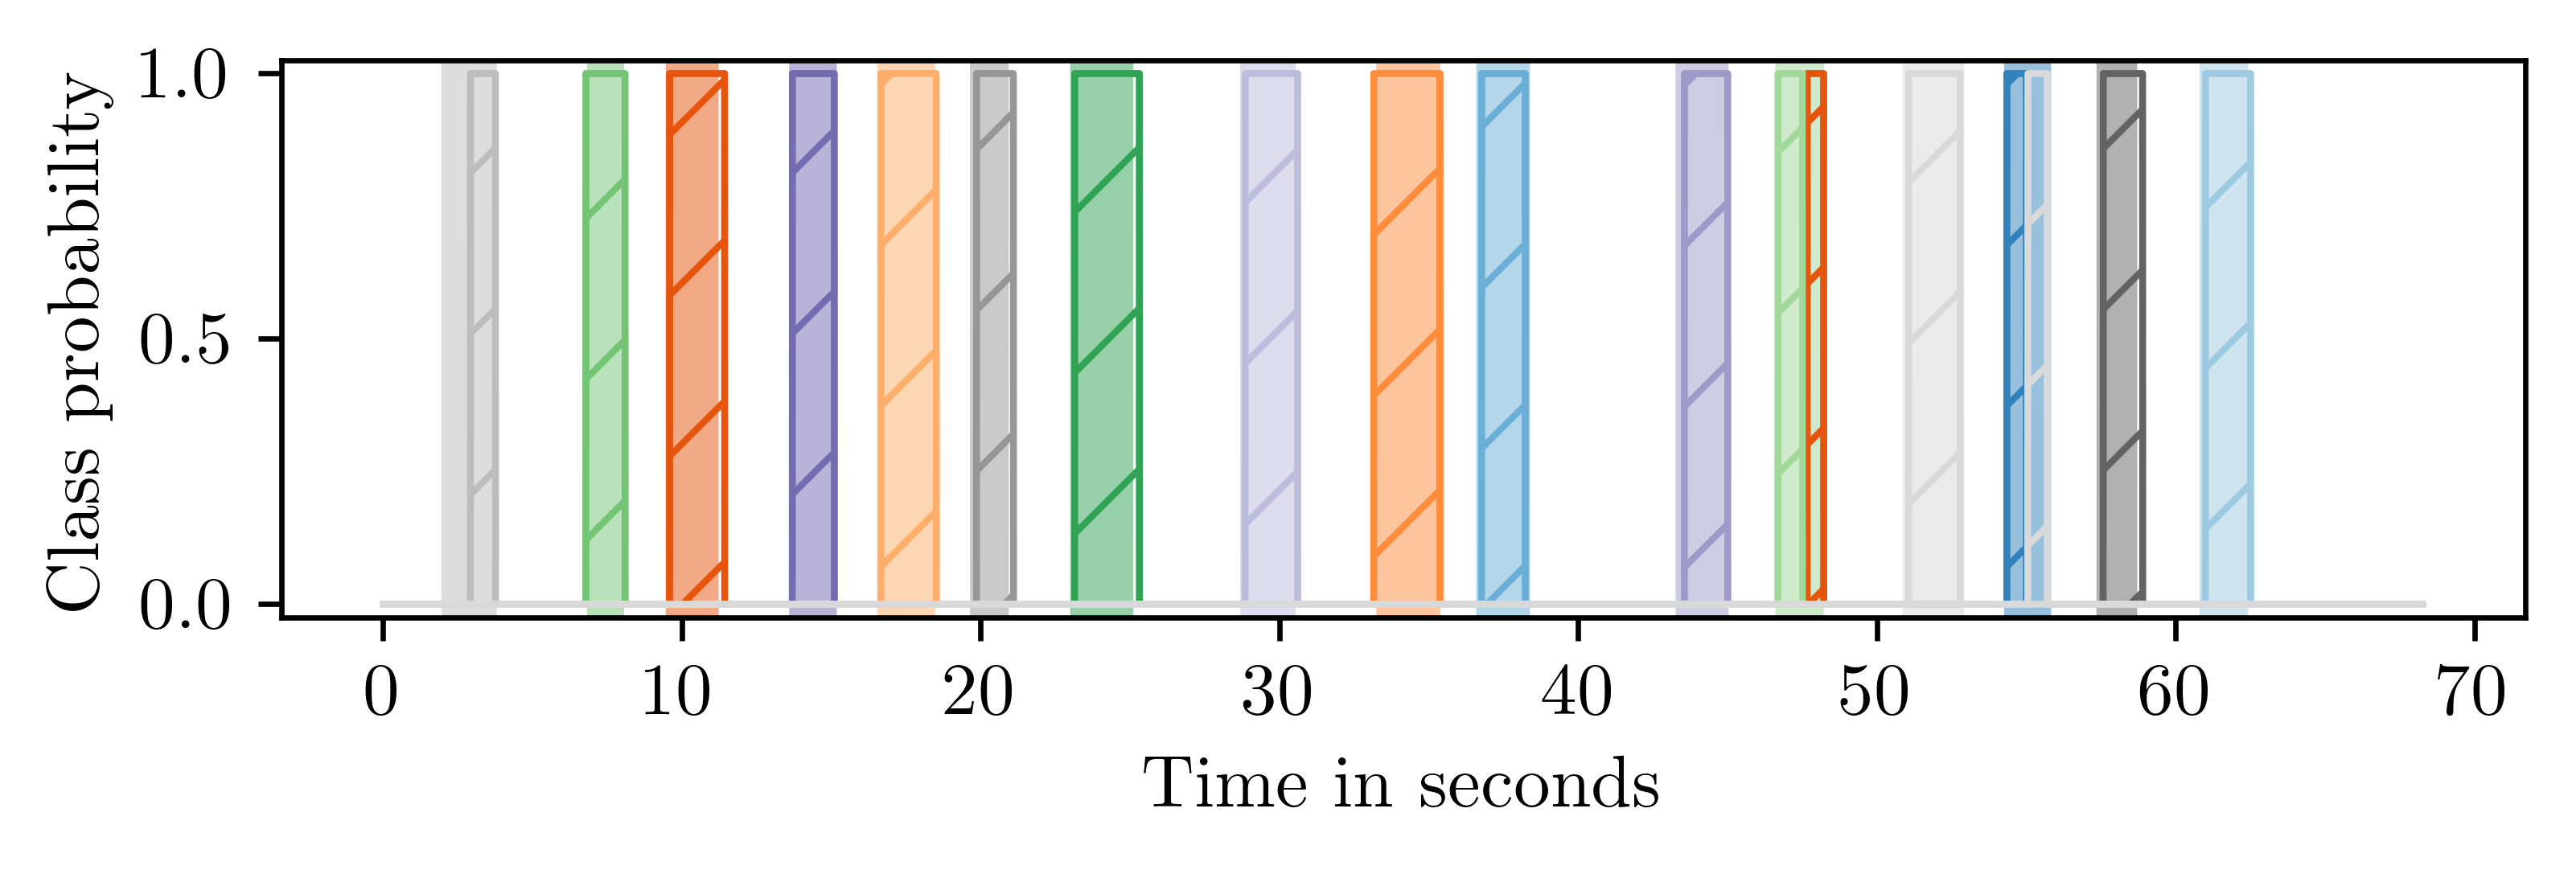
\includegraphics{figures/results/decoded/segmented}
    \caption{HMM segmentation plus segment decoding}
  \end{subfigure}
  \caption{Comparison of the two decoding methods on the same recording}
  \label{fig:decoded}
\end{figure}

\begin{figure}[h]
  \centering
  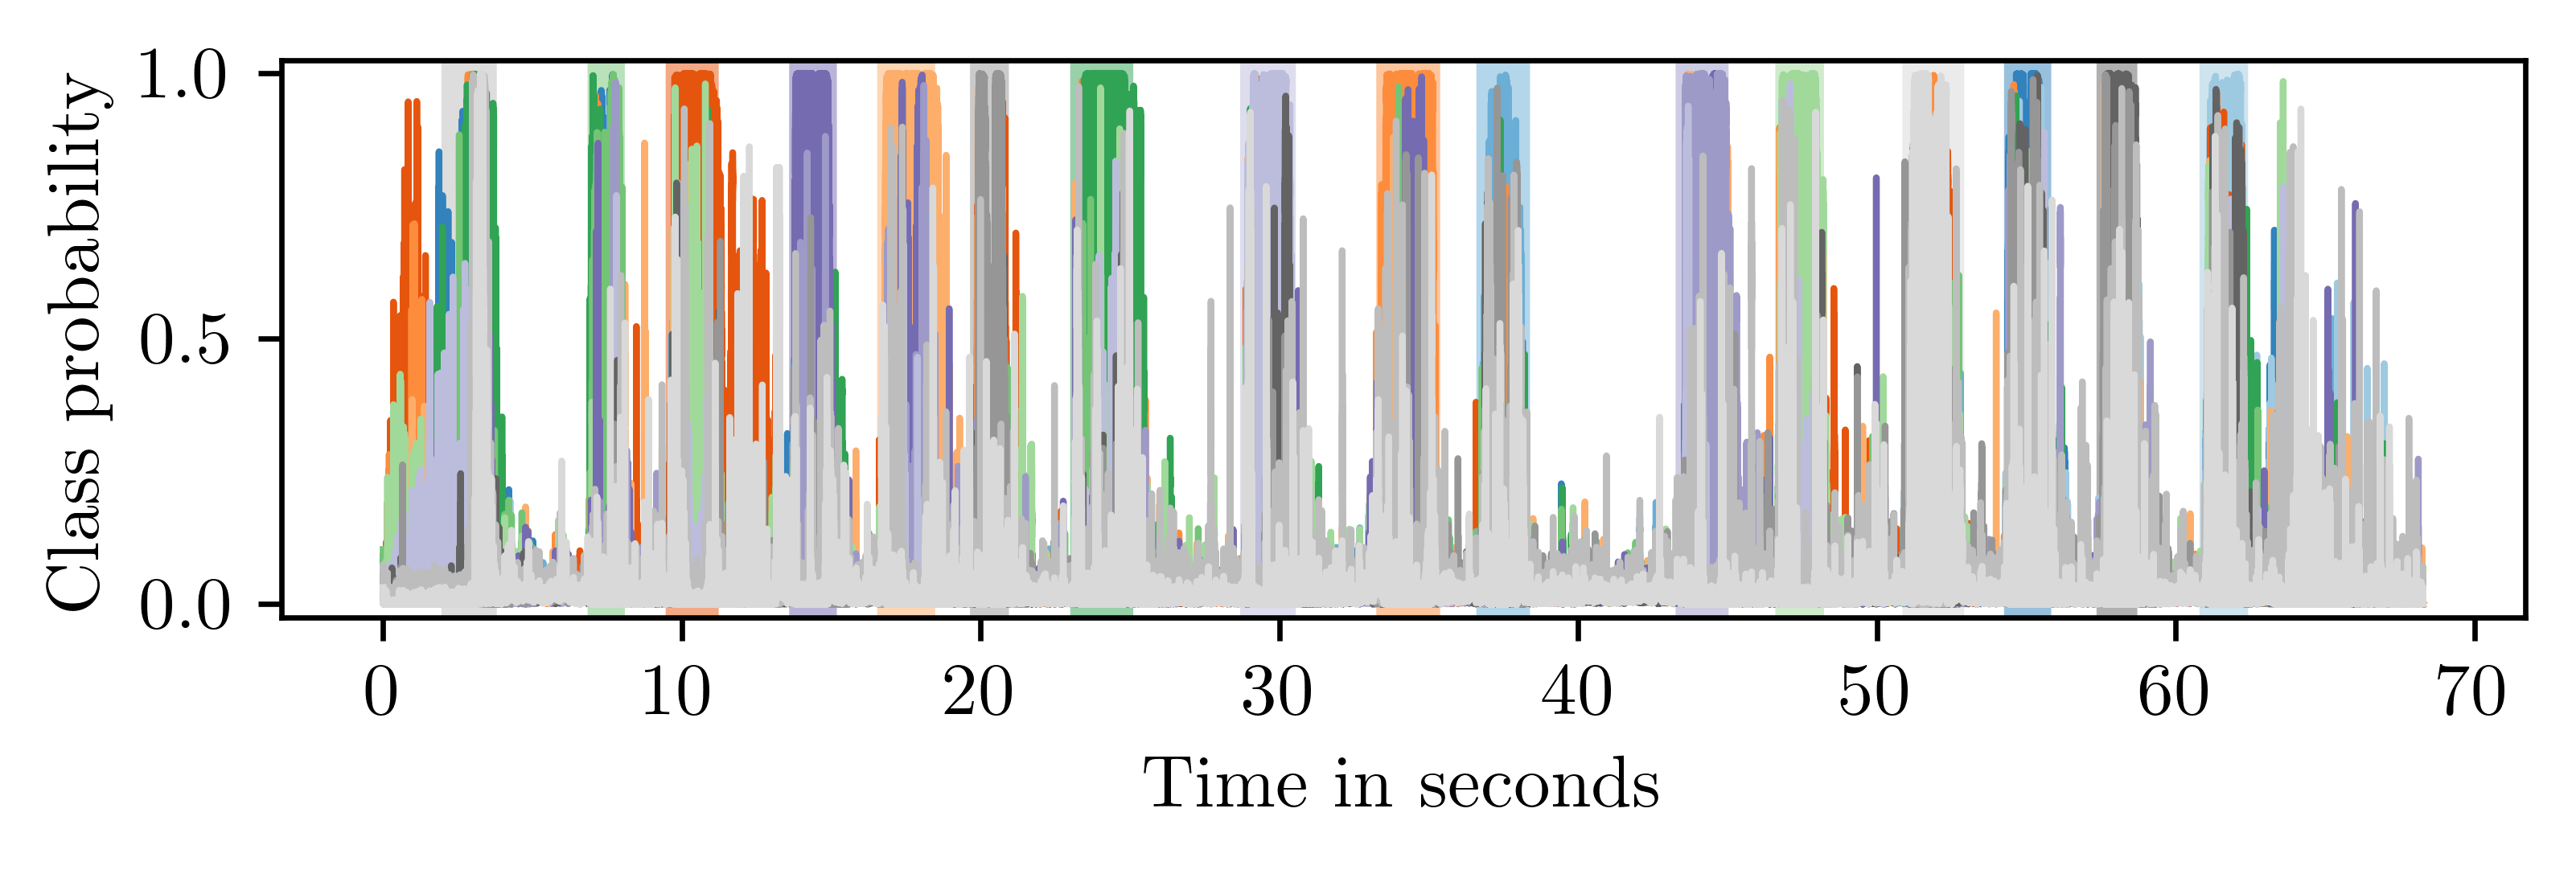
\includegraphics[width=6in]{figures/results/event-classifications.png}
  \caption{Noisy classifications produced by an RNN trained on event data}
  \label{fig:event-cls}
\end{figure}

The last thing to investigate is why the performance on InceptionV3 features
varies so little. However, that question is quickly answered by looking at the
classifier's confusion matrix in Figure \ref{fig:iv3-confusion} in comparison to
the confusion matrix of a framewise classifier for gists in Figure
\ref{fig:gists-confusion}. The training data was so uninformative that the
classifier just assigned everything to the most numerous class,
\texttt{<blank>}. Consequently, the output of any decoder is an empty or almost
empty sequence which has an edit distance of 16 to the ground truth.

\begin{figure}[h]
  \centering
  \begin{subfigure}{2.8in}
    \centering
    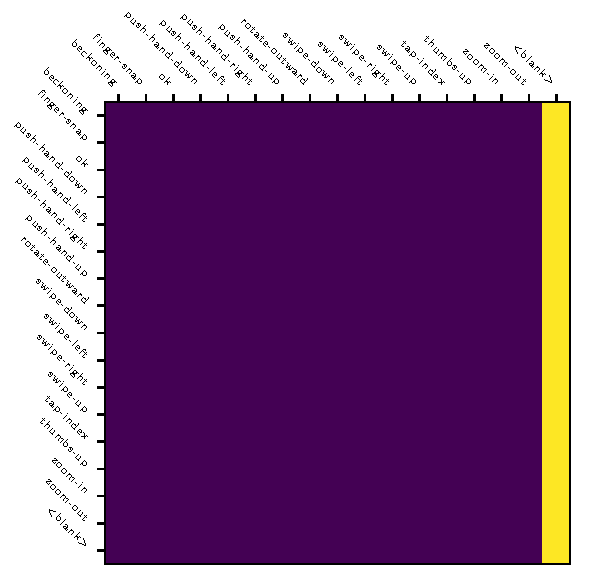
\includegraphics[width=\textwidth]{figures/results/confusion-matrices/ce/inceptionv3}
    \caption{Trained on InceptionV3 features}
    \label{fig:iv3-confusion}
  \end{subfigure}
  \hfill
  \begin{subfigure}{2.8in}
    \centering
    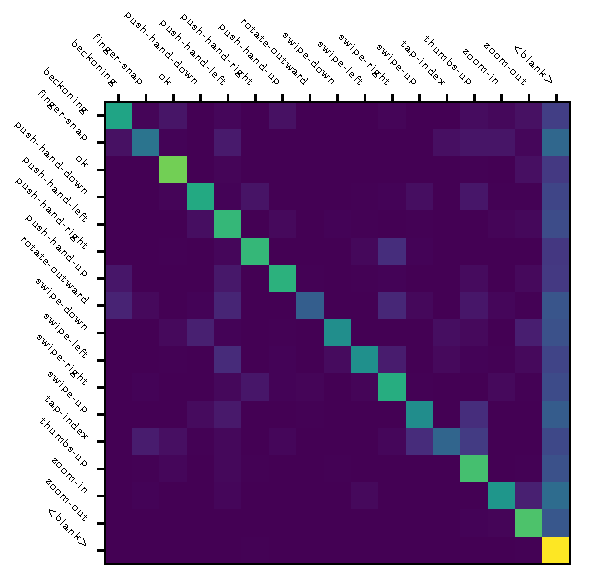
\includegraphics[width=\textwidth]{figures/results/confusion-matrices/ce/gists}
    \caption{Trained on gists}
    \label{fig:gists-confusion}
  \end{subfigure}
  \caption{Confusion matrices of framewise classifiers}
\end{figure}
